\subsection{Classic Planning Formalism}
\label{sec:pddl_formalism}
In this section, we will describe the methods that follow the classic task-planning formalism. Before introducing the methods, it is crucial to define the formalism with a set of foundational definitions.

Task-planning is a well-known problem that has been studied for many years. One of the most important formalization, still widely used today, is STRIPS (Stanford Research Institute Problem Solver) \cite{fikes1971strips}, which was developed in the 70s. STRIPS was initially an automated planning solver, but its primary contribution lies in its definition of a planning problem, which has served as the foundation for much of the research in subsequent decades.

According to the STRIPS formalism, a planning task is defined as a tuple $\Pi = (P, A, s_0, G, c)$, where:
\begin{itemize}
    \item $P$ is a set of propositions (also called facts).
    \item $A$ is a set of actions.
    \item A state $s$ is a subset of predicates, $s \subseteq P$, where $s_0$ is the initial state,
    \item $G \subseteq s$ represents the goal conditions.
    \item $c: A \leftarrow R$ is the cost function, which assign to an action $a \in A$ a real-value, $c(a)$ representing the cost of performing a given action.
\end{itemize}

An action $a \in A$ is defined as a tuple $a = \left(pre(a), add(a), del(a)\right)$, where $pre(a), add(a), del(a) \subseteq P$. These represent:
\begin{itemize}
    \item $pre(a)$: the preconditions (i.e., predicates that must be true to perform the action).
    \item $add(a)$: the added conditions (i.e., predicates that become true after the action is executed).
    \item $del(a)$: the deleted conditions (i.e., predicates that become false after the action is executed).
\end{itemize}
with the constraint that $add(a) \cap del(a) = \emptyset$. According to this formalism, an action is applicable in a state $s$ if $pre(a) \subseteq s$, and it results in the successor state $s' = (s \setminus del(a)) \cup add(a)$.

Building on these foundational concepts, the \textbf{Planning Domain Definition Language} (PDDL) was introduced in the 90s \cite{aeronautiques1998pddl}. PDDL is a human-readable format for describing automated planning problems. It provides a way to describe, the possible states of the world, the set of available actions, where each action description includes the prerequisites and the effects of the action, a specific initial state of the world and a specific set of desired goals. 

PDDL separates the model of a planning problem into two main components:
\begin{enumerate}
    \item The domain description, which defines the elements that are common across all problems within a given domain.
    \item The problem description, which specifies the specific planning problem, including the initial state and the goals to be achieved.
\end{enumerate}

\begin{figure}[t]
    \centering
    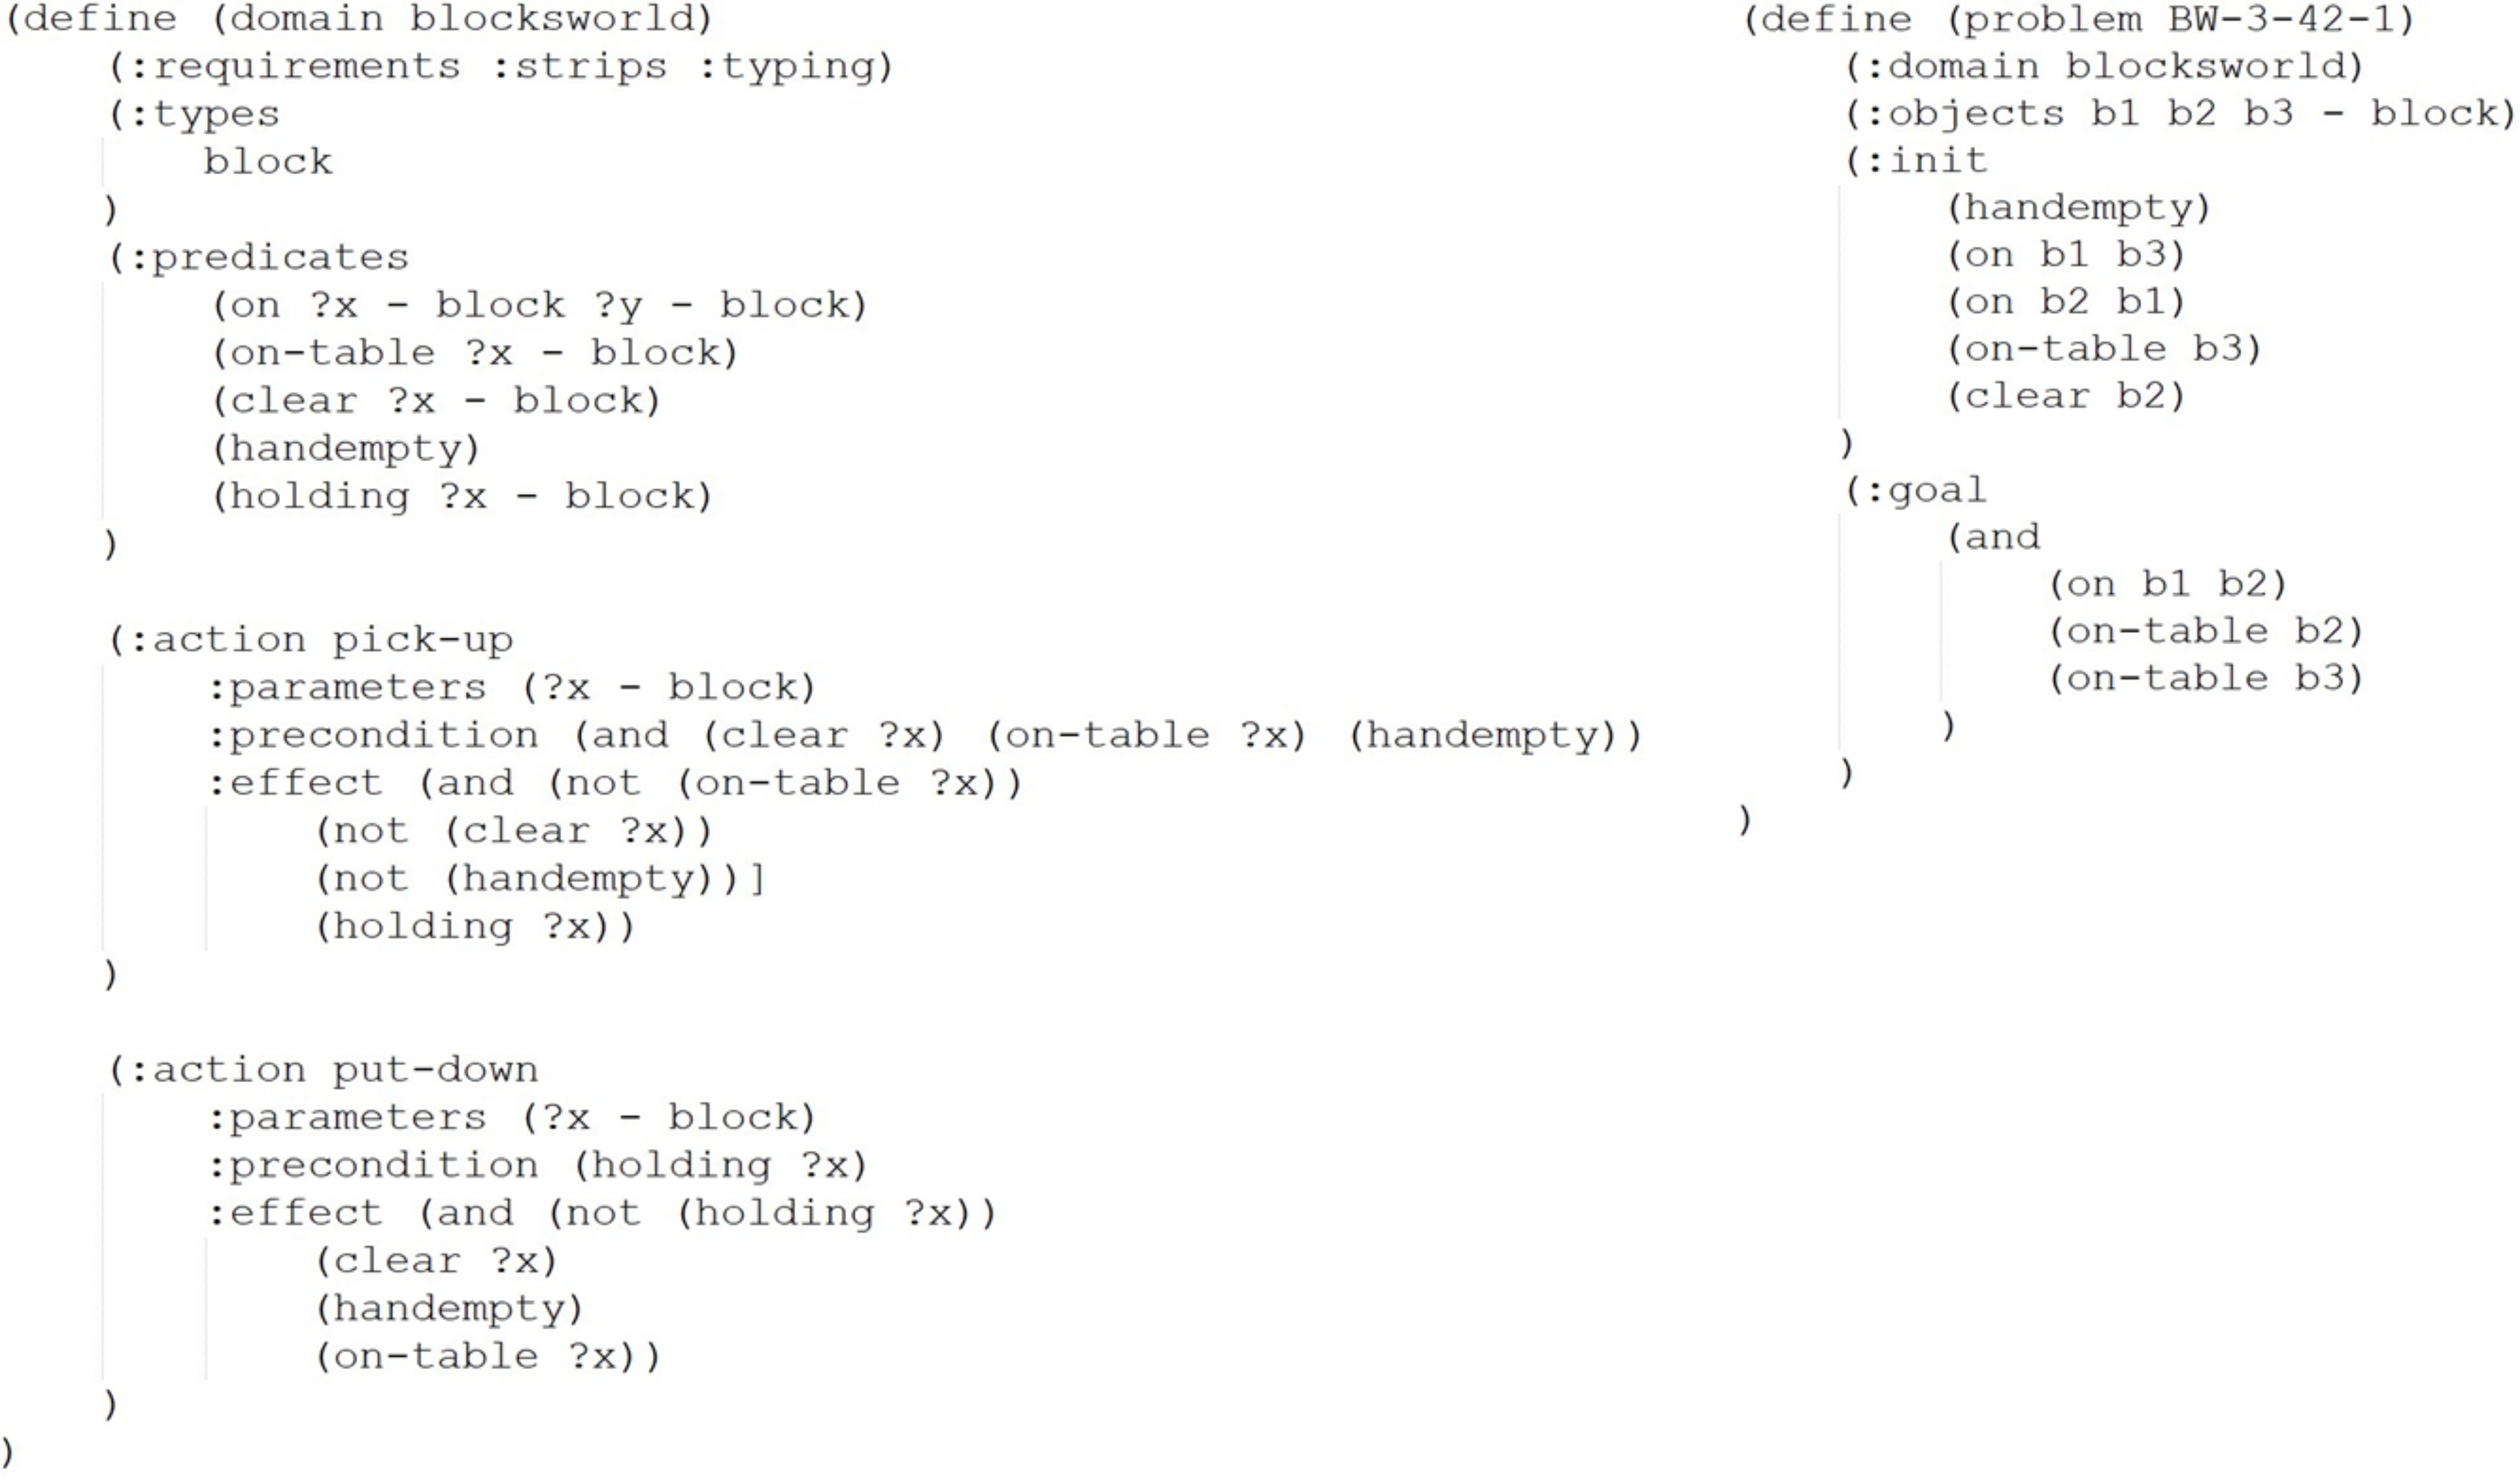
\includegraphics[width=1.0\textwidth]{figures/images/ch4/domain_problem.jpg}
    \caption{(Left) Example of a domain definition for the Blocks-World, specifying the predicates and actions available in the environment. (Right) Example of a problem definition for the domain, where a specific instance of the problem is defined, including object instances, the initial state, and the desired goal state.}
    \label{fig:domain_problem}
\end{figure}


Figure \ref{fig:domain_problem} provides examples of domain and problem definitions for the Blocks-World environment. As shown, when using the PDDL formalism, it is essential to fully define the elements of the world (e.g., blocks), the available actions (e.g., pick-up), along with their corresponding preconditions (i.e., predicates that must be true for the action to be executed) and postconditions (i.e., the effects of the actions). In the problem definition, specific instances of objects in the environment are specified, along with the initial state and goal state, both of which are defined based on the predicates available in the domain definition.

Once the problem is defined using the PDDL formalism, a complete parameterized instance must be specified to obtain a solution to the planning problem. This involves solving what is known as the \textbf{grounding problem}. During this process, all predicate and action variables must be instantiated with the objects defined in the problem. For instance, in the example shown in Figure \ref{fig:domain_problem}, the variable \( x \) is replaced with objects \( b1 \), \( b2 \), and \( b3 \) from the problem definition, leading to a complete enumeration of all predicates and actions. The result of this process is known as the \textit{Grounded Planning Problem}, which follows the same formalism as the STRIPS representation described earlier.

The grounded problem then serves as the input for planning algorithms, such as the well-known Fast Downward \cite{helmert2006fast} or LAMA \cite{richter2010lama}. While delving into the specifics of these algorithms is beyond the scope of this section, it is crucial to note that they are essentially \textit{search algorithms}. Given a state-space represented as a graph, which is derived from the Grounded STRIPS representation, these algorithms compute the (estimated) the shortest path in the state-space, connecting the source node (representing the initial state) to the target node (representing the goal state).

The limitations of these approaches have been well-known for a long time. Specifically, these algorithms do not scale well as the size of the problem (in terms of actions, predicates, and objects) increases. There are two main areas where higher problem dimensionality can cause performance issues:

\begin{enumerate}
    \item \textit{Search Phase}, as the dimensionality of the problem increases, the state-space expands correspondingly. This increases the time required to explore the state-space and find a solution path.
    \item \textit{Grounding Problem}, as the problem dimensionality grows, the time needed to generate a complete enumeration of all object combinations grows exponentially.
\end{enumerate}

To address the first issue, research has focused on developing methods to accelerate the search phase by introducing \textit{heuristics} that guide the search more efficiently towards the goal state. For the second issue, the literature has proposed methods that perform \textit{partial} grounding, concentrating on the action instances that are most relevant to the specific problem instance. Examples of these methods will be discussed in the following two paragraphs.

Here, a heuristic is a function $h: S \rightarrow \mathbb{R}$, which maps a state $s \in S$ to a real value $h(s)$, representing an estimate of the cost to reach the goal state from the state $s$. The optimal heuristic, denoted $h^{*}(s)$, is the heuristic that gives the exact cost of the optimal plan to reach a goal state from $s$. A heuristic is considered \textit{admissible} if it never overestimates the actual cost, i.e., $h(s) \leq h^{*}(s), \forall s \in S$. By utilizing the heuristic cost, a search algorithm can focus on exploring the most promising states instead of performing an exhaustive search of the entire state space.

In the context of task planning, a common heuristic is computed by solving the \textbf{Relaxed-STRIPS} problem. This is a simplified version of the STRIPS problem, where the delete conditions ($del$) are ignored, i.e., an action $a$ is represented as $a = \left(pre(a), add(a), \emptyset \right)$. The Relaxed-STRIPS problem is easier to solve because removing the $del$ conditions relaxes some of the constraints, allowing the state to include predicates that logically cannot be true simultaneously. By solving this relaxed problem, an estimated cost for reaching the goal from a given state can be computed. This approach has been used in well-known algorithms such as Fast-Downward \cite{helmert2006fast} and combined with novel heuristics in LAMA \cite{richter2010lama}.

\paragraph*{Heuristic Estimation}\mbox{}\\
In this paragraph the methods that propose GNN for computing heuristics estimation through the usage of GNNs are discussed. Specifically, the review will focus on two recent works \cite{shen2020learning,chen2024learning}.

The first remarkable work towards the use of GNN for heuristic estimation was proposed by authors of \cite{shen2020learning}. Here, authors started from the idea to leverage data-driven approaches to learn an heuristic function, and explore the possibility of such methods to generalize to different cardinalities and problems, and comparing the performance of such methods with classic heuristic functions.

The first step to solve this problem is related to the definition of the input. Specifically, the authors started by the Relaxed-STRIPS formulation. The STRIPS problem can be easily formulated as a graph if the following observations are done:
\begin{itemize}
    \item A node, can be described a predicate which can be either a pre-condition or an added condition.
    \item The edge is represented by the action that connects the pre-conditions to the added-conditions. 
\end{itemize}
\begin{figure}[t]
    \centering
    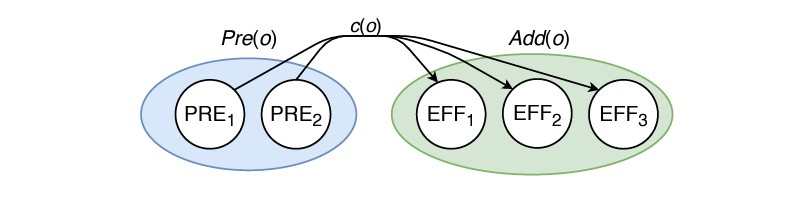
\includegraphics[width=1\textwidth]{figures/images/ch4/nodes_mapping.jpg}
    \caption{Example of nodes and edges definition in \cite{shen2020learning}. The hyper-edge represents an action that connects multiple nodes. The sending nodes are preconditions, while the receiver nodes are the effects.}
    \label{fig:nodes_mapping}
\end{figure}

Figure \ref{fig:nodes_mapping} illustrates the mapping of predicates and actions to graph nodes and edges. As can be observed, an action connects multiple nodes. To model this, the authors use a generalized graph structure known as a \textit{hypergraph}. Formally, a hypergraph is defined as a triple $G = (u, V, E)$, where $V = \left\{ \textbf{v}_{i}: i \in \left\{1, 2, \dots, N^{v} \right\} \right\}$ is the set of $N^{v}$ vertices, and $E = \left\{ (e_{k}, R_{k}, S_{k}): k \in \left\{1, 2, \dots, N^{e} \right\} \right\}$ is the set of $N^{e}$ hyper-edges. In this structure, $R_{k}$ is the receiver set, containing the indices of the nodes for which the $k$-th edge acts as an incoming edge, and $S_{k}$ is the sender set, containing the indices of the nodes for which the $k$-th edge acts as an outgoing edge. Then, $\textbf{v}_{i}$ is the node embedding, which has been implemented as a binary-vector $v_i = [x_s, x_g]$, where $x_s, x_g \in \left\{0,1\right\}$. $x_s=1$ iff the i-th predicate is true in the state s and $x_g=1$ iff the predicate is true in the goal-state. While, $e_{k}$ is the edge embedding, $e_k = [c(a_k), |Pre(a_k)|, |Add(a_k)|]$, where $c(a_k)$ is the cost of the operator, $|Pre(a_k)|$ is the number of pre-condition and $|Add(a_k)|$ is the number of added condition.

\begin{figure}[t]
    \centering
    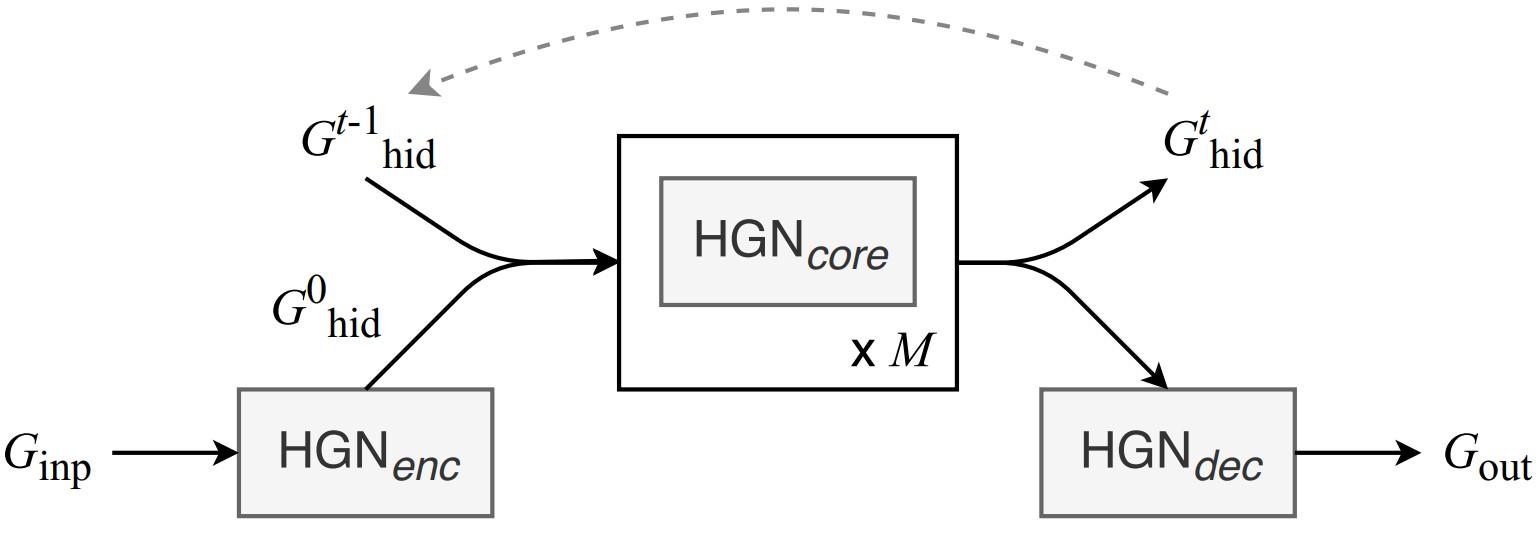
\includegraphics[width=0.8\textwidth]{figures/images/ch4/strips_hgn_architecture.jpg}
    \caption{Architecture of the STRIPS-HGN model \cite{shen2020learning}. The model is composed of three main components: the encoder, the hyper-graph network, and the decoder. The encoder processes the input graph, generating a first hidden graph representation. The HGN implements the message passing mechanism, updating the hidden graph representation. The decoder generates the output graph, which global value represents the predicted heuristic.}
    \label{fig:strips_hgn_architecture}
\end{figure}

\begin{figure}[t]
    \centering
    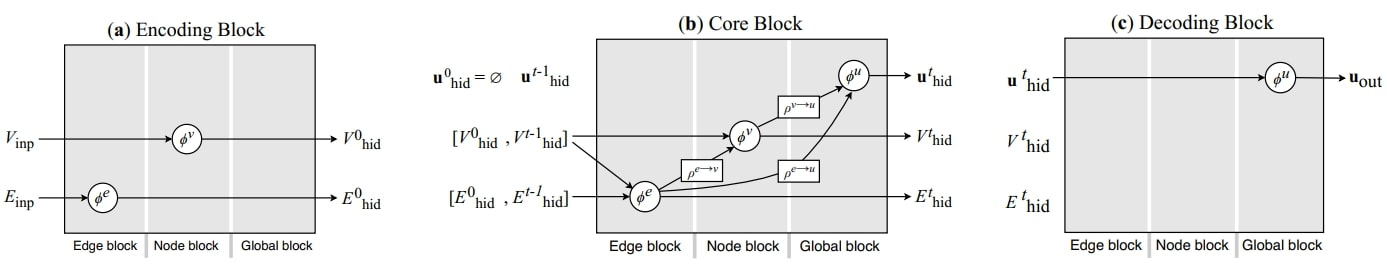
\includegraphics[width=1.0\textwidth]{figures/images/ch4/computational_flow.jpg}
    \caption{Computational flow of the STRIPS-HGN model \cite{shen2020learning}, consisting of three main blocks: Encoding, Core, and Decoding. The Encoding Block generates initial hidden representations for both node and edge embeddings. The Core Block implements the message-passing mechanism, updating the hidden representations of nodes, edges, and global embeddings. Finally, the Decoding Block generates the output graph, where the global embedding represents the predicted heuristic value.}
    \label{fig:computation_flow}
\end{figure}

Once the graph structure has been defined, the module that processes this input can be described. Specifically, the authors propose leveraging the concept behind the \textit{Interaction Network} \cite{battaglia2016interaction}. The architecture, depicted in Figure \ref{fig:strips_hgn_architecture}, implements the computational flow shown in Figure \ref{fig:computation_flow}, and can be divided into the following three steps.

\begin{enumerate}
    \item The \textit{Encoding Block} consists of two functions, $\phi^{e}$ and $\phi^{v}$, both implemented as Multi-Layer Perceptrons (MLPs). These functions transform the initial binary inputs into higher-dimensional representations, specifically, $\phi^{e}(e_j)$ produces $e_{hid}^{0}$ and $\phi^{v}(v_i)$ produces $v_{hid}^{0}$, where both $e_{hid}^{0}$ and $v_{hid}^{0} \in \mathbb{R}^{32}$. This step expands the original binary vectors (of size 2 or 3) into 32-dimensional vectors.

    \item The \textit{Core Block} implements the Message-Passing Iterative Procedure and is divided into the following steps:

        \begin{enumerate}
            \item \textit{Edge Block}: For each edge (representing an action), $e_{hid,j}^{t-1}$ is generated by concatenating the embeddings of the receiver and sender nodes associated with the edge. An MLP encoder is then applied to this concatenated information to create a new edge representation $e_{hid,j}^{t}$.

            \item \textit{Node Block}: Similar to the Interaction Network, only the receiver nodes' states are updated. The edge information influencing each receiver is aggregated by summing the embeddings of the incoming edges using the function $\rho^{e \rightarrow v}$. The node input is constructed by concatenating the incoming edge embeddings $e_{hid,j}^{t}$, the initial node embedding $v_{hid,i}^{0}$, and the previous node state $v_{hid,i}^{t-1}$. This concatenated input is then passed through an MLP to generate the updated node representation $v_{hid,i}^{t}$.

            \item \textit{Global Block}: This block updates the global graph representation by aggregating both node and edge embeddings using the functions $\rho^{e \rightarrow u}$ and $\rho^{v \rightarrow u}$, respectively. The aggregated information is passed through an MLP to produce the new global graph representation.
        \end{enumerate}

    \item The \textit{Decoding Block} acts as a decoder, implemented as an MLP. It takes the updated global graph representation as input and generates a heuristic value for a given state, aiding in the decision-making process.
\end{enumerate}

The operations in the core block are repeated for $M$ iterations, where $M = 10$ in this work.
The system is trained by minimizing the loss function defined in Equation \ref{equation:loss_func}. Here, $h^{*}(s)$ represents the ground truth heuristic value for state $s$, obtained by solving the training planning problem with a classical planning algorithm.
\begin{equation}
    \mathcal{L}_\theta(\mathcal{B})=\frac{1}{|\mathcal{B}|} \sum_{\left(G, h^*(s)\right) \in \mathcal{B}} \frac{1}{M} \sum_{t \in \{1, \ldots, M\}}\left(h_t^\theta(G)-h^*(s)\right)^2
    \label{equation:loss_func}
\end{equation}

Interesting results were obtained during the experiments. Notably, the system demonstrated the ability to learn both domain-dependent heuristics (when tested on the same domain it was trained on) and domain-independent heuristics (when tested on a different domain). This shows that the trained GNN was capable of generating meaningful heuristic values that could be effectively used by search algorithms like A*. However, a general drawback of this approach is the time required to compute the heuristic, particularly when the model is run on a CPU instead of a GPU, which significantly impacts performance.

The development of such work was proposed by \cite{chen2024learning}. In this work, the authors conducted a comprehensive analysis of learned heuristics in relation to problem representation. Specifically, they introduced three distinct representations for the planning problem:

\begin{itemize}
    \item \textit{STRIPS Learning Graph} (SLG): This is a graph constructed from the STRIPS representation. Compared to the representation used in \cite{shen2020learning}, the main improvement lies in the use of labeled edges, which can now represent all edge types, namely, preconditions, added conditions, and deleted conditions.
    
    \item \textit{Finite Domain Representation Learning Graph} (FLG): This graph is built from the Finite Domain Representation. In this framework, nodes represent both facts (tuples of state variables $v_i$ and values $d \in D_v$) and actions, while edges represent the relationships between facts and actions, such as preconditions and effects.
    
    \item \textit{Lifted Learning Graph} (LLG): This representation avoids the grounding phase entirely. To achieve this, the authors proposed a schema consisting of two main components: the \textit{Action Schema} and the \textit{Instance Subgraph}. The Action Schema encodes domain-specific information, where nodes represent predicates, argument indices, and variables. The Instance Subgraph encodes specific information about the current state and goal state, where nodes represent predicates, states, goal arguments, and objects.
\end{itemize}

Using these representations, the authors trained a GNN architecture to learn the heuristic function across the three different representations. The results demonstrated that the proposed method was capable of learning both \textit{domain-dependent} and \textit{domain-independent} heuristics. However, when analyzing the coverage performance, i.e., the number of problems solved within a 10-minute timeout, it became clear that performance varied significantly depending on the problem domain. The classic feed-forward heuristic outperformed the GNN-based \\ heuristic in 3 out of 8 domains, while the GNN-based heuristic outperformed the feed-forward heuristic in 4 out of 8 domains. One domain showed equal performance between the two approaches. Notably, the GNN-based heuristic struggled with the domain-independent test scenarios, meaning that the model was not able to generalize well to unseen domains. This limitation represents a significant drawback, as one of the most important assumptions behind the use of GNNs, or data-driven approaches in general, is their ability to generalize to novel scenarios.

\paragraph*{Grounding Problem}\mbox{}\\
As stated earlier, one of the preliminary challenges to address before running the search algorithm is the \textit{Grounding Problem}, which involves computing all valid instantiations that assign objects to the arguments of predicates and action parameters.

It is important to note that the size of the grounded task grows exponentially with the number of arguments in the predicates and action schemas. Although this size remains constant for all tasks within a given domain, and grounding can be computed in polynomial time, it may still become prohibitive when the number of objects is large and/or when some predicates or actions have many parameters. This issue is particularly problematic in open multi-task environments, where many objects exist, but only a few are relevant to the task at hand.

The authors in \cite{gnad2019learning} build upon these observations and propose an algorithm that performs \textit{partial grounding}. The main idea of this approach is to focus on the action instances most relevant to the specific problem instance. In this context, the challenge lies in how to identify and select the most relevant actions for grounding. To address this, a \textit{priority function}, $f: O \rightarrow \left[0, 1\right]$, is learned, where $O$ is the set of all operators, and $f(o)$ represents the priority of operator $o$.

This priority function is learned using a supervised learning approach, with the training dataset defined as \\ $\mathcal{D} = \left\{s_{0}, G, \Sigma^{O}, o, \left\{0,1\right\} \right\}$. Here, $s_{0}$ is the initial state, $G$ is the goal state, $\Sigma^{O}$ is the set of objects, $o \in O$ is the operator, and $\left\{0,1\right\}$ is the label, where $1$ indicates that the operator is part of an optimal path, and $0$ otherwise.

The authors trained a Support Vector Regression (SVR) model, representing the operators with \textit{Relational Rules} (RR). Each operator is associated with a set of rules that are instantiated by grounding the operator's variables. The operator is then represented by a binary feature vector, where each element corresponds to a rule, with a value of $1$ if the rule is satisfied, and $0$ otherwise. The SVR is trained to predict the priority of an operator based on its binary feature vector.

The system was evaluated on problems where the size of grounded instances grows cubically with respect to the parameters of the generator, resulting in large instances that are difficult to fully ground. The model was trained on smaller problem instances, where full grounding could be computed in a reasonable time. During testing, the model was evaluated on larger instances. Results showed that the learned partial-grounding approach using SVR-RR was able to solve 255 out of 313 problems, outperforming the fully grounded approach, which solved only 156 out of 313 problems.

However, no discussion on the quality of the generated plans was provided. In fact, an evolution of these methods was proposed at the ICAPS 2023 Planning Competition \cite{gzubicki2023huzar}. Results from the competition, however, revealed that these learning-based methods are still significantly behind classical grounding methods, both in terms of optimality and computation time.
